%%%%%%%%%%%%%%%%%%%%%%%%%%%%% Define Article %%%%%%%%%%%%%%%%%%%%%%%%%%%%%%%%%%
\documentclass{article}
%%%%%%%%%%%%%%%%%%%%%%%%%%%%%%%%%%%%%%%%%%%%%%%%%%%%%%%%%%%%%%%%%%%%%%%%%%%%%%%

%%%%%%%%%%%%%%%%%%%%%%%%%%%%% Using Packages %%%%%%%%%%%%%%%%%%%%%%%%%%%%%%%%%%
\usepackage{listings, xcolor}
\usepackage{parskip}
\usepackage{hyperref}
\usepackage{amsmath}
\usepackage{graphicx}
\usepackage[a4paper, margin = 1.5cm]{geometry}
\usepackage{float}
\usepackage{amssymb}

%%%%%%%%%%%%%%%%%%%%%%%%%%%%%%% Title & Author %%%%%%%%%%%%%%%%%%%%%%%%%%%%%%%%
\title{UML}
\author{Trentin Tommaso}
%%%%%%%%%%%%%%%%%%%%%%%%%%%%%%%%%%%%%%%%%%%%%%%%%%%%%%%%%%%%%%%%%%%%%%%%%%%%%%%

\begin{document}
  \maketitle
  \tableofcontents
  \newpage
  \section{Introduzione}
    \subsection{Motivazione}
      Moderni sistemi SW tendono a crescere e diventare sempre più complessi $\rightarrow$ impensabile comprenderli direttamente dal codice. Nasce quindi necessità di forme dio rappresentazione astratte $\rightarrow$ nascita \textbf{modellazione}.  
    \subsection{Terminologia}
      \begin{itemize}
        \item \textbf{Modello}: astrazione che descrive sistema / sottosistema;
        \item \textbf{Vista}: descrizione degli aspetti fisici di un sistema da una certa prospettiva (si omettono dettagli non rilevanti);
        \item \textbf{Notazione}: insieme di elementi grafici / testuali e refole per rappresentare le viste.
      \end{itemize}
    \subsection{Linguaggi di modellazione}
      In passato erano utilizzati diversi linguaggi di modellazione, negli ultimi anni si sta affermando UML (Unified Modelling Language) come linguaggio unificato per essere utilizzato in tutte le atttività di modellazione. 
      \subsubsection{UML: Idea}
        Famiglia di notazioni grafiche che si basano su un singolo \textbf{meta-modello} (modello che definisce concetti stessi del linguaggio di modellazione, indica seconfo quali regole sia possibile costruire modelli UML). UML \textit{non è una metodologia}: il suo obiettivo è fornire un supporto al processo di sviluppo SW. 
    \subsection{Regole Prescrittive / Descrittive}
      \begin{itemize}
        \item Regole \textbf{prescrittive}: stabilite da organismi standardizzanti che definiscono precisamente lessico, sintassi e semantica del linguaggio;
        \item Regole \textbf{descrittive}: stabilite per convenzione comune, possono essere meglio comprese guardando come UML viene usato nella pratica da un'organizzazione;
      \end{itemize}
      Bisogna conoscere sempre convenzioni particolati della specifica organizzazione e del singolo progetto, anche se al di fuori dello standard.
    \subsection{UML: Utilizzi}
      \begin{itemize}
        \item \textbf{Bozza}: tracciare modello informale di un sistema da realizzare (\textit{forward engineering}) o per descrivere sistemi esistenti (\textit{reverse engineering});
        \item \textbf{Progetto dettagliato (blueprint)}: realizzare un modello completo della soluzione architetturale del sistema;
        \item \textbf{Linguaggio di programmazione}: in grado di modellare completamente e precisamente il sistema SW. 
      \end{itemize}
      \subsubsection{Bozze: Espressività > Completezza}
        Scopo: aiutare comunicazione e discussione idee, esplorando soluzioni alternative, diagrammi non devono essere esaustivi / definire tutti gli aspetti del codice. Vengono spesso disegnate collaborativamente in poco tempo, non rispettando tutte le regole formali dello standard. 
      \subsubsection{Progetto Dettagliato: Espressività + Completezza}
        Scopo: aiutare comprensione e completezza. Progettista sviluppa modello di progetto che sviluppatore dovrà realizzare (salvandolo in file condivisi). Completezza e non ambiguità aiutano il programmatore che verrà guidato dal modello e non dovrà interpretarne aspetti ambigui. 
      \subsubsection{Linguaggio di Programmazione}
        Approccio \textbf{MDA} (Model Driven Architecture) esplora la possibilità di usare UML come linguaggio di programmazione, volendo stabilire una sintassi e una semantica per UML in modo da portare a generazione automatica di codice eseguibile rappresentativo del modello. Sfida: modellare precisamente anche la logica del progetto, Vantaggio: generazione codice per diverse piattaforme target parteno da un modello indipendente dalla piattaforma.
    \subsection{Informazioni Soppresse}
      Assenza di qualche informazione da un diagramma UML non implica, in generale, che tale informazione non esista (alcuni aspetti potrebbero essere assenti perché non ancora trattati al momento della stesura del diagramma). 
    \subsection{Tipi di Diagrammi}
      UML 2 possiede 13 tipi differenti di diagrammi ufficiali, appartenenti a due categorie:
      \begin{itemize}
        \item \textbf{Diagrammi strutturali}: modellano organizzazione del sistema;
        \item \textbf{Diagrammi comportamentali}: modellano comportamento e interazioni tra le entità del sistema.
      \end{itemize}
      Tali diagrammi rappresentano i deliverables di diverse fasi del ciclo di vita del SW, tra cui analisi di requisiti e attività di progettazione di alto / basso livello. 
      \begin{figure}[h!]
        \begin{center}
          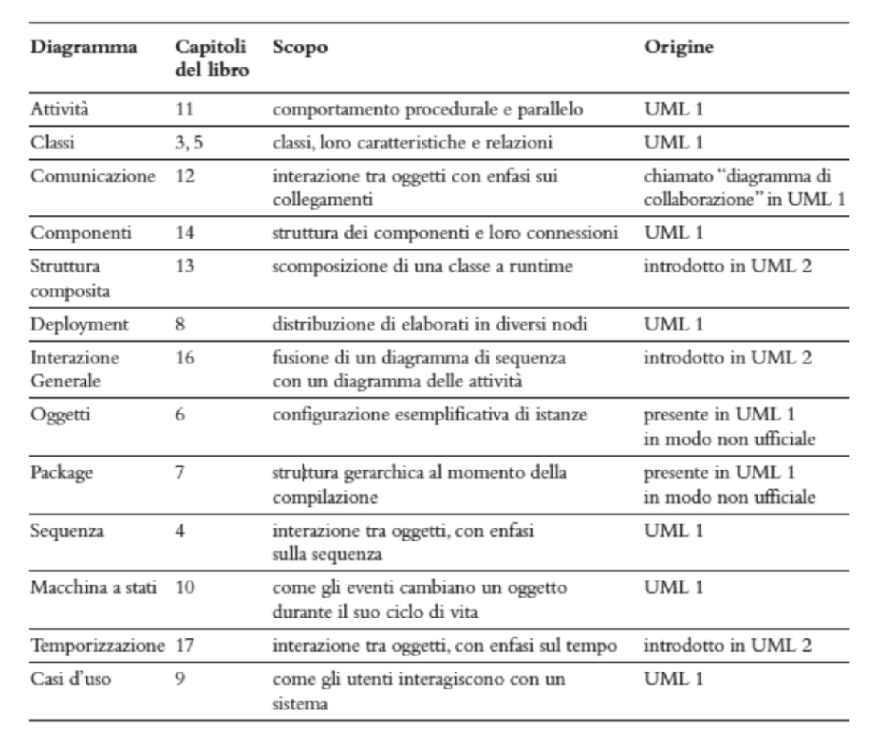
\includegraphics[width=0.5\textwidth]{figures/uml_t.png}
        \end{center}
      \end{figure}
    \subsection{Integrazione nel Processo di Sviluppo}
      \begin{itemize}
        \item \textbf{Analisi dei requisiti}: facilita deduzione dei requisiti, notazione non deve essere troppo complessa per favorire comunicazione con cliente;
        \item \textbf{Progettazione}: modelli più tecnici / dettagliati per descrivere sistema a ingegneri che lo devono implementare;
        \item \textbf{Documentazione}: modelli rendono più semplice la descrizione di parti complesse o convogliano messaggi intuitivamente e immediatamente;
        \item \textbf{Comprensione di SW pre-esistente}: evoluzione / reverse engineering.
      \end{itemize}
      Nei processi iterativi ogni iterazione arricchisce i diagrammi delle iterazioni precedenti.
\end{document}
